\chapter{Random-Hierarchy Ablation for CIFAR-100 Curriculum Learning}
\label{app:hierarchy-ablation-curriculum}

\section{Purpose}

Appendices~\ref{app:cifar100-model-size-curriculum} and
\ref{app:roughness-followup-curriculum} showed that the fixed coarse-to-fine
curriculum is most useful for the weaker CIFAR-100 CNNs. The remaining question
was whether this gain actually depends on the learned class hierarchy, or
whether it is mostly caused by reducing the number of labels during the first
training stage.

This appendix tests that point directly. The learned hierarchy is compared with
random hierarchies that preserve the same tree shape. In other words, the random
condition keeps the same number of hierarchy levels and the same cluster sizes,
but permutes which CIFAR-100 classes belong to those clusters. This makes the
comparison stricter than using an arbitrary random tree: the schedule and the
amount of label coarsening are matched, while the semantic or model-derived
class grouping is destroyed.

\section{Protocol}

The ablation uses the strongest cheap setting from the earlier appendices:
CIFAR-100, \texttt{cnn\_w0.5}, Adam with learning rate 0.001, batch size 128,
100 epochs, and a fixed 20-epoch curriculum. The learned hierarchy is built from
the baseline model's last-layer classifier-weight geometry, treating class
weight vectors as class embeddings. The random hierarchies are random
permutations of this learned hierarchy.

The experiment contains 15 finished runs:

\begin{itemize}
    \item three baselines, using seeds 42, 43, and 44,
    \item three learned-hierarchy curriculum runs, one per training seed,
    \item nine random-hierarchy curriculum runs, using three random hierarchy
          seeds for each training seed.
\end{itemize}

The main comparison is the learned hierarchy against the mean of the three
random hierarchies for the same training seed. The best random hierarchy per
seed is also reported as an optimistic diagnostic. That value answers a stronger
question: even if several random hierarchies were tried and the best one was
kept, would it match the learned hierarchy?

\section{Main result}

Table~\ref{tab:hier-ablation-aggregate} summarizes the ablation. Accuracy values
are means over training seeds and are shown as percentages. Gains are percentage
points relative to the matching baseline.

\begin{table}[h]
\centering
\small
\begin{tabular}{lrrrr}
\hline
Condition & Best acc. & Best gain & Final acc. & AUC gain \\
\hline
Baseline & 35.29 & -- & 32.01 & -- \\
Learned hierarchy & 37.53 & +2.24 & 32.75 & -3.83 \\
Random hierarchy mean & 35.81 & +0.53 & 31.75 & -5.39 \\
Best random hierarchy & 36.34 & +1.05 & -- & -- \\
\hline
\end{tabular}
\caption{CIFAR-100 \texttt{cnn\_w0.5} hierarchy ablation. The random mean first
averages the three random hierarchies within each training seed and then
averages across seeds. AUC is computed over the test-accuracy trajectory.}
\label{tab:hier-ablation-aggregate}
\end{table}

The learned hierarchy clearly outperforms the random hierarchy control. It
improves best test accuracy by +2.24 percentage points, while the average random
hierarchy improves it by only +0.53 points. The learned hierarchy beats the
random mean for all three training seeds. Even the best of the three random
hierarchies per seed reaches only +1.05 points on average, still well below the
learned hierarchy.

This means that the curriculum benefit is not explained only by reducing the
number of labels during early training. Random coarsening can give a small gain,
so the reduced-label effect is real, but most of the improvement in this setting
comes from using a class grouping aligned with the trained model's classifier
geometry.

\begin{figure}[h]
    \centering
    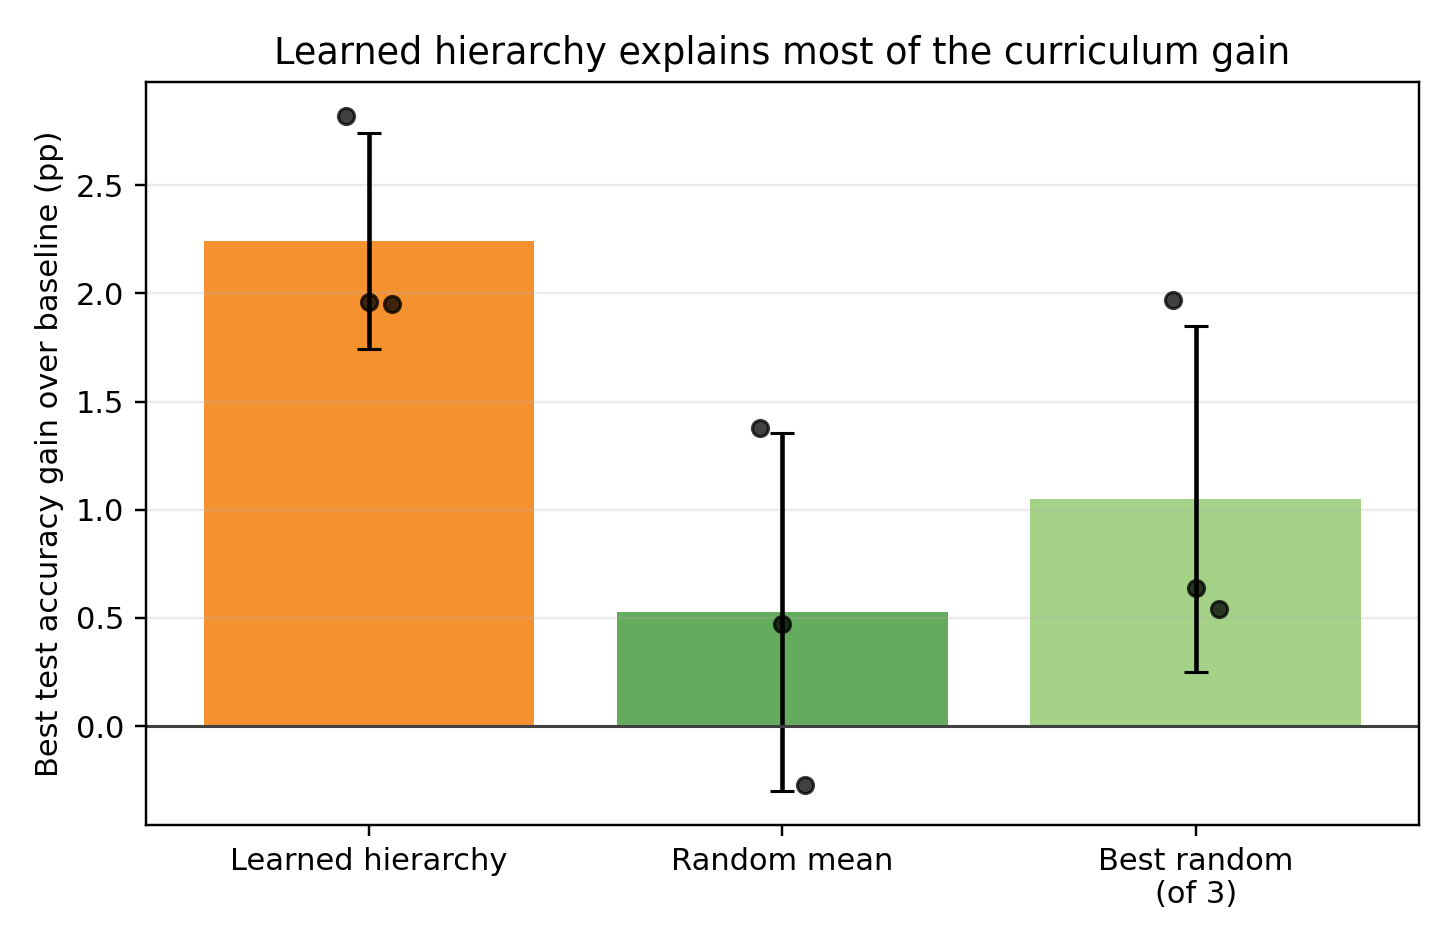
\includegraphics[width=0.82\textwidth]{figures/hierarchy_ablation_gain_comparison.png}
    \caption{Best test-accuracy gain over the matching baseline for learned and
    random hierarchies. Black points show the three training seeds. The learned
    hierarchy beats both the random mean and the best-of-three random diagnostic.}
    \label{fig:hier-ablation-gain-comparison}
\end{figure}

\section{Per-seed behavior}

Table~\ref{tab:hier-ablation-seeds} gives the paired seed-level results. The
learned hierarchy is consistently better than the random mean. The gap is
smallest for seed 42 and largest for seed 44, where the random mean is slightly
worse than the baseline.

\begin{table}[h]
\centering
\small
\begin{tabular}{rrrrrr}
\hline
Seed & Baseline & Learned & Random mean & Best random & Learned - random \\
\hline
42 & 34.98 & 37.80 & 36.36 & 36.95 & +1.44 \\
43 & 35.42 & 37.38 & 35.89 & 36.06 & +1.49 \\
44 & 35.46 & 37.41 & 35.19 & 36.00 & +2.22 \\
\hline
Mean & 35.29 & 37.53 & 35.81 & 36.34 & +1.72 \\
\hline
\end{tabular}
\caption{Seed-level best test accuracy for the hierarchy ablation. All values
except the last column are percentages. The last column is the learned-hierarchy
advantage over the random-hierarchy mean in percentage points.}
\label{tab:hier-ablation-seeds}
\end{table}

\section{Learning curves}

Figure~\ref{fig:hier-ablation-learning-curves} shows the test-accuracy
trajectories. The random curve is averaged within each training seed before
averaging across seeds, so the shaded region does not treat the nine random runs
as nine independent training seeds.

\begin{figure}[h]
    \centering
    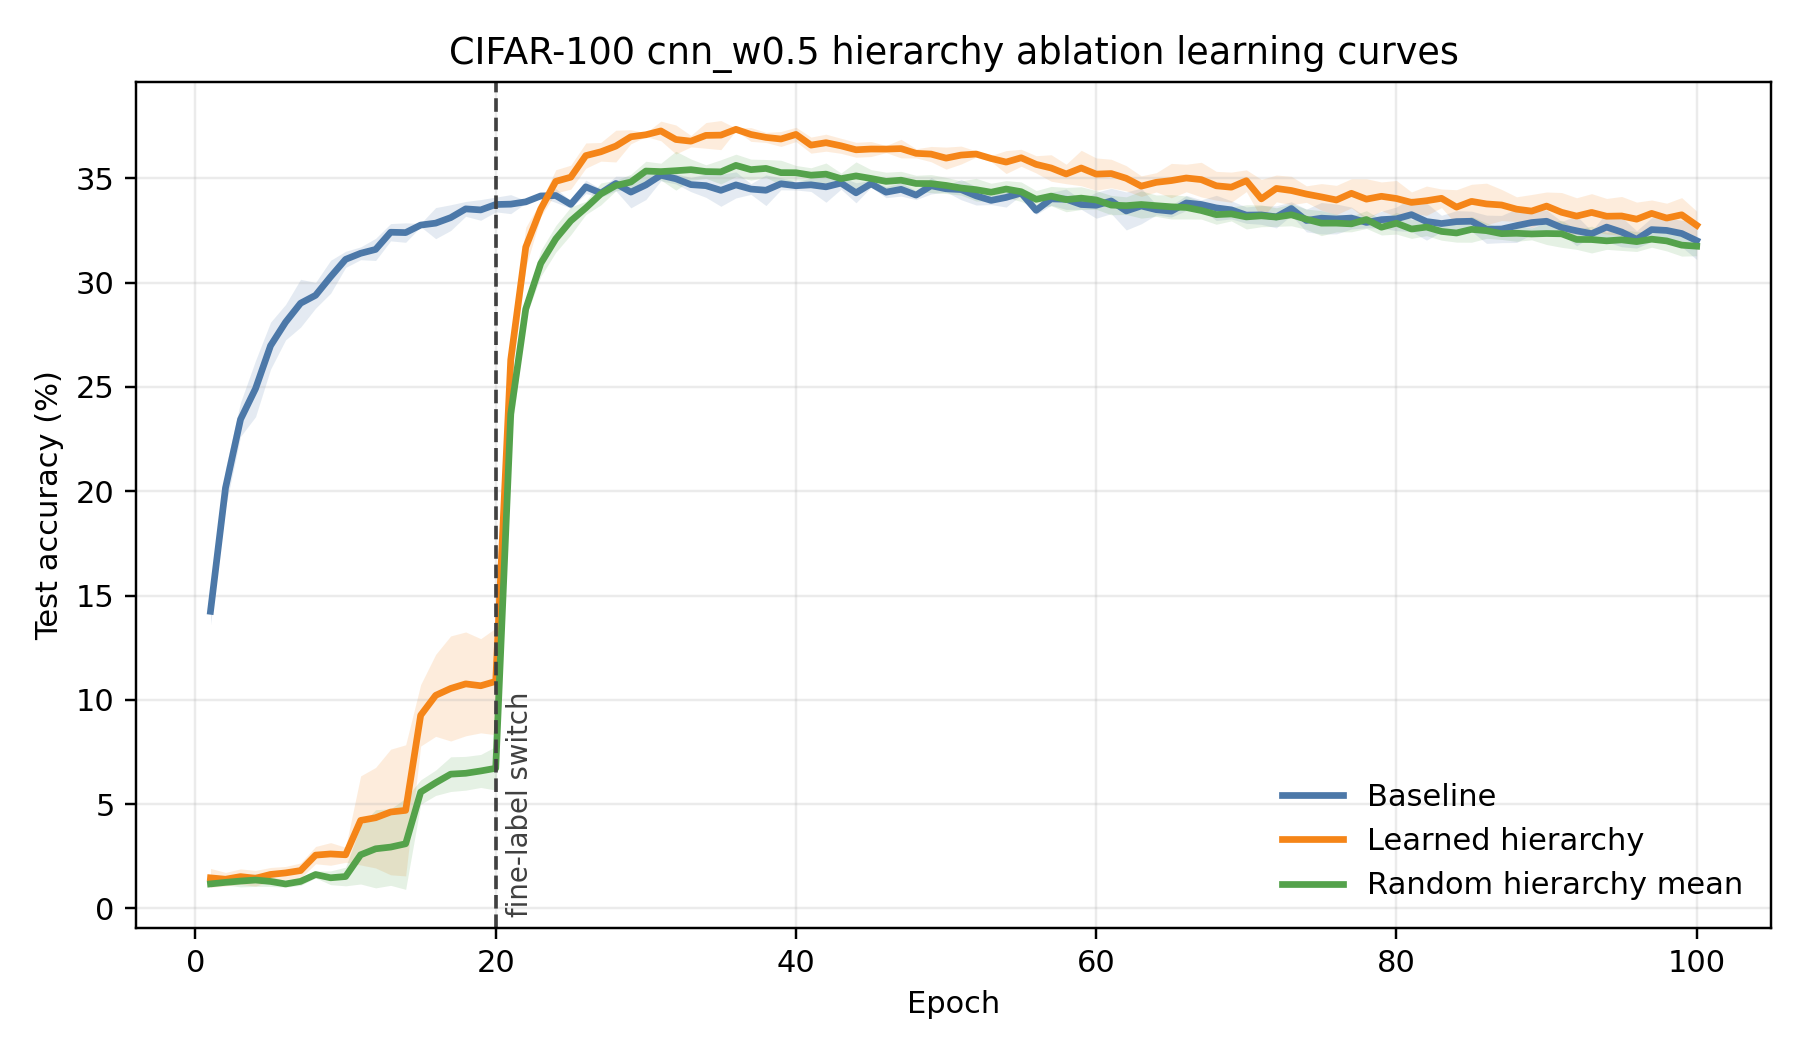
\includegraphics[width=0.90\textwidth]{figures/hierarchy_ablation_learning_curves.png}
    \caption{Learning curves for the CIFAR-100 hierarchy ablation. The vertical
    dashed line marks the switch from coarse labels to fine labels after 20
    epochs. Both curriculum variants pay an early fine-label accuracy cost, but
    the learned hierarchy recovers to a higher peak than the baseline and the
    random hierarchy.}
    \label{fig:hier-ablation-learning-curves}
\end{figure}

The trajectory confirms the interpretation from the previous appendices. The
curriculum is not a faster way to train this model: the learned-hierarchy AUC is
3.83 percentage points below baseline, and the random-hierarchy AUC is 5.39
points below baseline. The benefit is instead a higher peak after the fine-label
phase begins. The learned hierarchy provides a better warm-up than random
coarsening, while the random hierarchy mostly adds delay.

\section{Relation to the previous curriculum results}

Table~\ref{tab:hier-ablation-previous-context} places the ablation next to the
main CIFAR-100 \texttt{cnn\_w0.5} results from
Appendix~\ref{app:roughness-followup-curriculum}. The exact baselines differ
slightly because these are separate W\&B run groups, but the scale of the effect
is consistent.

\begin{table}[h]
\centering
\small
\begin{tabular}{lrrl}
\hline
Experiment/method & Best acc. & Gain & Role \\
\hline
This appendix: baseline & 35.29 & -- & ablation reference \\
This appendix: learned fixed \texttt{curr20} & 37.53 & +2.24 & hierarchy test \\
This appendix: random fixed \texttt{curr20} & 35.81 & +0.53 & random control \\
Appendix G: fixed \texttt{curr20} & 37.58 & +2.54 & previous best fixed schedule \\
Appendix G: adaptive all levels & 37.19 & +1.75 & adaptive schedule \\
Appendix G: adaptive max1 & 37.22 & +2.24 & hierarchy-depth test \\
\hline
\end{tabular}
\caption{Comparison with previous CIFAR-100 \texttt{cnn\_w0.5} results. Values
are percentages and percentage-point gains. Appendix G rows are shown for
context, not as part of the random-hierarchy ablation.}
\label{tab:hier-ablation-previous-context}
\end{table}

The ablation strengthens the earlier conclusion that hierarchy quality matters.
Appendix~\ref{app:roughness-followup-curriculum} showed that hierarchy depth and
schedule length matter; this appendix shows that the class grouping itself also
matters. The learned hierarchy is not merely a convenient way to create fewer
labels. Its grouping carries useful information for the curriculum.

\section{Conclusion}

For the strongest CIFAR-100 weak-CNN setting, the generated classifier-weight
hierarchy explains most of the curriculum gain. Random hierarchies with matched
cluster sizes give only a small improvement and remain below the learned
hierarchy even under a best-of-three random diagnostic. This does not prove that
the classifier-weight hierarchy is optimal, and it does not test all datasets or
architectures. It does, however, close the main missing ablation from
Appendix~\ref{app:roughness-followup-curriculum}: the positive CIFAR-100 result
is not just an artifact of training first on fewer labels.
